%%
% Modificación de una plantilla de Latex para adaptarla al castellano.
%%

%%%%%%%%%%%%%%%%%%%%%
% Thin Sectioned Essay
% LaTeX Template
% Version 1.0 (3/8/13)
%
% This template has been downloaded from:
% http://www.LaTeXTemplates.com
%
% Original Author:
% Nicolas Diaz (nsdiaz@uc.cl) with extensive modifications by:
% Vel (vel@latextemplates.com)
%
% License:
% CC BY-NC-SA 3.0 (http://creativecommons.org/licenses/by-nc-sa/3.0/)
%
%%%%%%%%%%%%%%%%%%%%%

%----------------------------------------------------------------------------------------
%	PACKAGES AND OTHER DOCUMENT CONFIGURATIONS
%----------------------------------------------------------------------------------------

\documentclass[a4paper, 10pt]{article} % Font size (can be 10pt, 11pt or 12pt) and paper size (remove a4paper for US letter paper)
\usepackage{helvet}
\renewcommand{\familydefault}{\sfdefault}
\usepackage[protrusion=true,expansion=true]{microtype} % Better typography
\usepackage{graphicx} % Required for including pictures
\usepackage[usenames,dvipsnames]{color} % Coloring code
\usepackage{wrapfig} % Allows in-line images
\usepackage[utf8]{inputenc}
\usepackage{enumerate}
\usepackage{enumitem}

% Imágenes
\usepackage{graphicx} 

\usepackage{amsmath}
% para importar svg
%\usepackage[generate=all]{svgfig}

% sudo apt-get install texlive-lang-spanish
\usepackage[spanish]{babel} % English language/hyphenation
\selectlanguage{spanish}
% Hay que pelearse con babel-spanish para el alineamiento del punto decimal
\decimalpoint
\usepackage{dcolumn}
\newcolumntype{d}[1]{D{.}{\esperiod}{#1}}
\makeatletter
\addto\shorthandsspanish{\let\esperiod\es@period@code}
\makeatother

\usepackage{longtable}
\usepackage{tabu}
\usepackage{supertabular}

\usepackage{multicol}
\newsavebox\ltmcbox

% Para algoritmos
\usepackage{algorithm}
\usepackage{algorithmic}
\usepackage{amsthm}

% Para matrices
\usepackage{amsmath}

% Símbolos matemáticos
\usepackage{amssymb}
\usepackage{accents}
\let\oldemptyset\emptyset
\let\emptyset\varnothing

\usepackage[hidelinks]{hyperref}

\usepackage[section]{placeins} % Para gráficas en su sección.
\usepackage[T1]{fontenc} % Required for accented characters
\newenvironment{allintypewriter}{\ttfamily}{\par}
\setlength{\parindent}{0pt}
\parskip=8pt
\linespread{1.05} % Change line spacing here, Palatino benefits from a slight increase by default

\makeatletter
\renewcommand\@biblabel[1]{\textbf{#1.}} % Change the square brackets for each bibliography item from '[1]' to '1.'
\renewcommand{\@listI}{\itemsep=0pt} % Reduce the space between items in the itemize and enumerate environments and the bibliography
\newcommand{\imagen}[2]{\begin{center} \includegraphics[width=90mm]{#1} \\#2 \end{center}}
\newcommand{\RFC}[1]{\href{https://www.ietf.org/rfc/rfc#1.txt}{RFC-#1}}

\renewcommand{\maketitle}{ % Customize the title - do not edit title and author name here, see the TITLE block below
\begin{center} % Center align
{\Huge\@title} % Increase the font size of the title
\end{center}

\vspace{20pt} % Some vertical space between the title and author name

\begin{flushright} % Right align
{\large\@author} % Author name
\\\@date % Date

\vspace{40pt} % Some vertical space between the author block and abstract
\end{flushright}
\renewcommand{\baselinestretch}{0.5}

}
%----------------------------------------------------------------------------------------
%	TITLE
%----------------------------------------------------------------------------------------

\title{\textbf{Ingeniería de Servidores\\Práctica 4: Benchmarks}\\ % Title
\vspace{20 pt}
Cuestiones de la Práctica 4} % Subtitle

\author{\textsc{Adrián Portillo Sánchez} % Author
\\{\textit{Universidad de Granada}}} % Institution

\date{\today} % Date

%----------------------------------------------------------------------------------------
\setcounter{secnumdepth}{0}
\usepackage{anysize}
\marginsize{3cm}{3cm}{2.5cm}{2.5cm}

\begin{document}
\thispagestyle{empty}
\maketitle
\pagebreak
\thispagestyle{empty}
\tableofcontents
\pagebreak
\listoffigures
\pagebreak

\section{Cuestión 1}
\textbf{Instale Phoronix Suite, seleccione un benchmark de entre los disponibles, descárguelo y ejecútelo. Describa el propósito del benchmark y su interés en el mismo. Explique razonadamente el significado de los resultados obtenidos.}\\

Lo primero que deberemos hacer es instalar la aplicación “Phoronix Test Suite” \cite{1}, tanto en Ubuntu Server como en CentOS podremos instalarla directamente con el gestor de paquetes que usemos.

En el caso de Ubuntu Server deberemos introducir
\begin{verbatim}
# sudo apt-get install phoronix-test-suite
\end{verbatim}

\begin{figure}[H]
\centering 
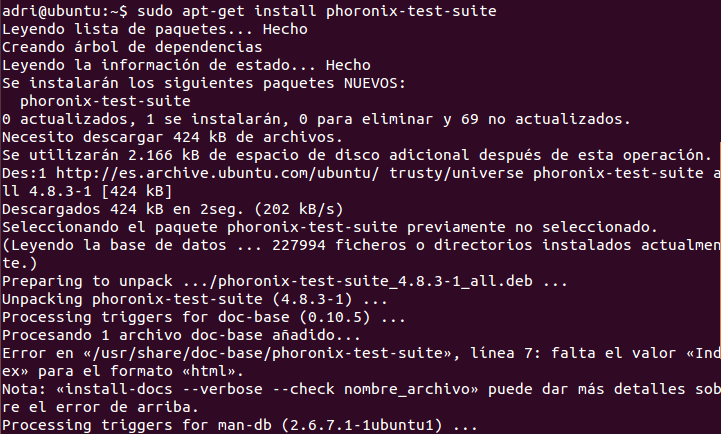
\includegraphics[width=1\linewidth]{phoronix1.png} 
\caption{Instalando Phoronix Suite en Ubuntu Server.} 
\label{contexto:figura} 
\end{figure}

En el caso de CentOS en primer lugar descargamos Phoronix Suite de la web oficial \url{http://www.phoronix-test-suite.com/?k=downloads} y seleccionaremos el paquete
genérico que posteriormente descomprimiremos y ejecutaremos desde terminal el archivo \textbf{'installsh'}.
Una vez se ha realizado esto podremos ejecutar Phoronix si tenemos las dependencias de
php necesarias según la web solo es necesario el paquete \textit{'php5-cli'}, sin embargo puede ser que
se tengan que instalar las dependencias una a una dependiendo de la que falte como es mi caso, faltaba DOM y fue necesaria la ejecución de:
\begin{verbatim}
# sudo yum install php-xml
\end{verbatim}

\begin{figure}[H]
\centering 
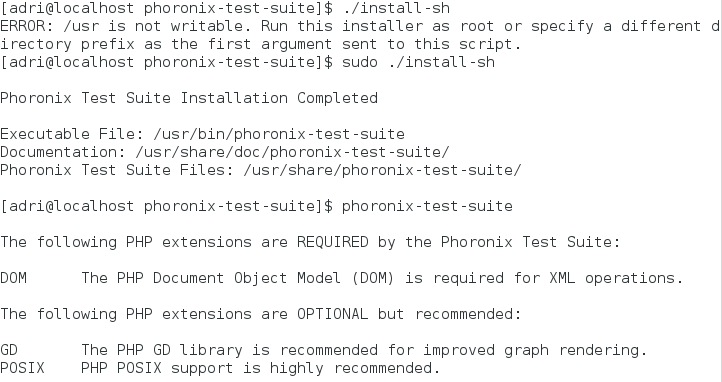
\includegraphics[width=1\linewidth]{phoronix2.png} 
\caption{Instalando Phoronix Suite en CentOS.} 
\label{contexto:figura} 
\end{figure}

Una vez instaladas las dependencias ejecutamos phoronix con el comando \textit{'phoronix-test-suite'} y completamos algunas opciones de configuración\cite{3}. Antes de poder realizar los test, debemos conocer qué benchmarks están disponibles, por lo que necesitamos una lista con todos los test disponibles. Para listar los benchmarks disponibles introducimos en el terminal: 
\begin{verbatim}
# phoronix-test-suite list-tests
\end{verbatim}

\begin{figure}[H]
\centering 
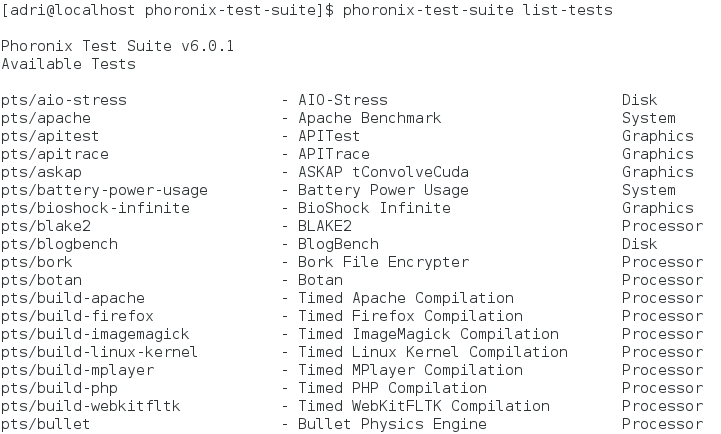
\includegraphics[width=1\linewidth]{phoronix3.png} 
\caption{Lista de Benchmarks de Phoronix.} 
\label{contexto:figura} 
\end{figure}

\section{Cuestión Opcional 1.}
\textbf{Seleccione, instale y ejecute uno, comente los resultados. Atención: no es lo mismo un benchmark que una suite, instale un benchmark.}\\

Viendo la lista de benchmarks decidimos el benchmark que vamos a utilizar\cite{4}, en nuestro caso usaremos \textit{'pts/apache'}, por lo que es necesario aplicar el siguiente comando: \textit{'phoronix-test-suite install pts/apache'} y comenzara a instalar el benchmark, por último para usarlo solo es necesario el comando \textit{'phoronix-test-suite benchmark pts/apache'}

En los resultados obtenemos que se han realizado 4637.51 peticiones por segundo (figura 4), además se muestra el error normal de 72.93 y la desviación típica 3.15\%; Se usan peticiones por segundo debido a que el benchmark de apache consiste en realizar peticiones al servidor HTTP GET (concurrentemente también) para ver cuanto es el tiempo de respuesta, esto permite realizar una comparación de servidores apache, en un futuro incluso se podría realizar un benchmark con distintos protocolos web como HTTP2 y ver que protocolo funciona mejor con apache.

\begin{figure}[H]
\centering 
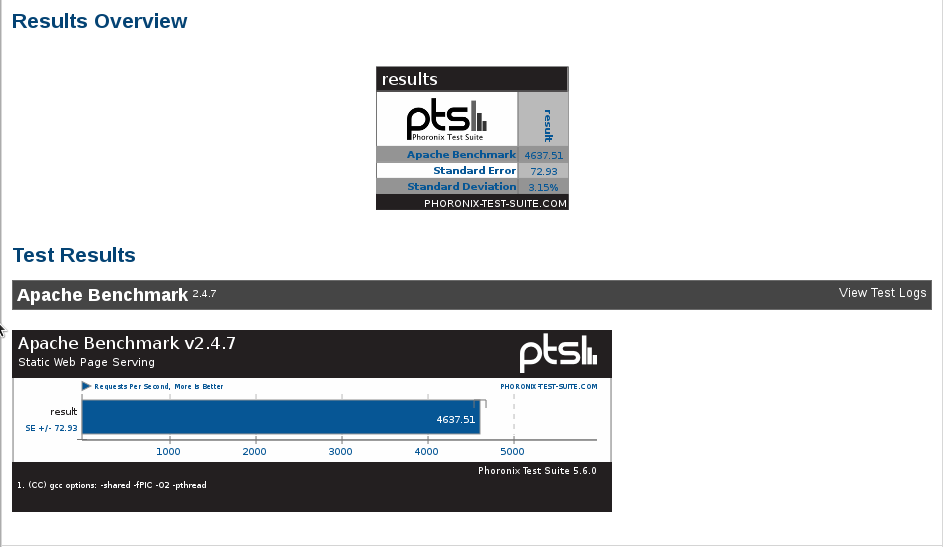
\includegraphics[width=1\linewidth]{phoronix4.png} 
\caption{Resultados benchmark apache.} 
\label{contexto:figura} 
\end{figure}

\pagebreak

\section{Cuestión 2.}
\textbf{De los parámetros que le podemos pasar al comando ¿Qué significa -c 5? ¿y -n 100? Monitorice la ejecución de ab contra alguna máquina (cualquiera) ¿cuántos procesos o hebras crea ab en el cliente?}\\

El parámetro \textit{'-c'} indica la concurrencia\cite{5}, pasar como parámetro \textit{'-c 30'}, indicará que vamos ejecutar concurrentemente 30 solicitudes a la vez.
\begin{verbatim}
-c concurrency
Number of multiple requests to perform at a time. Default is one request at a time.
# Número de solicitudes a realizar al mismo tiempo. Por defecto se realiza una a cada vez.
\end{verbatim}
El parámetro \textit{'-n'} indica el número de solicitudes, usar \textit{'-n 1000'} significará que le vamos a hacer 1000 solicitudes al servidor.
\begin{verbatim}
-n requests
Number of requests to perform for the benchmarking session. The default is to just
perform a single request which usually leads to non-representative benchmarking results.
# Número de solicitudes a realizar para la sesión de benchmarking.Por defecto se 
# realiza una sola solicitud lo que suele llevar a resultados no representativos.
\end{verbatim}

\section{Cuestión 3.}
\textbf{Ejecute ab contra a las tres máquinas virtuales (desde el SO anfitrión a las máquina virtuales de la red local) una a una (arrancadas por separado) y muestre y comente las estadísticas. ¿Cuál es la que proporciona mejores resultados? Fíjese en el número de bytes transferidos, ¿es igual para cada máquina?}\\

Para hacer las pruebas a todos los servidores de las máquinas virtuales en igual de condiciones, ejecutaremos ab desde nuestro sistema operativo anfitrión\cite{5}, como en nuestro caso es Windows 7, vamos a descargarnos XAMPP, que ya contiene los ejecutable de Apache y podremos usarlos sin tener que hacer ninguna instalación, lo descargaremos desde \url{http://www.apachefriends.org/download.php?xampp-portable-lite-win32-1.8.1-VC9.zip} y podremos ejecutar directamente Apache Benchmark, que se encuentra dentro de la carpeta \textit{'apache/bin'}.

\pagebreak

Hechas las pruebas a los servidores de las 3 máquinas virtuales los resultados son los siguientes:

\begin{itemize}
\item Benchmark del Apache en CentOS.

\begin{figure}[H]
\centering 
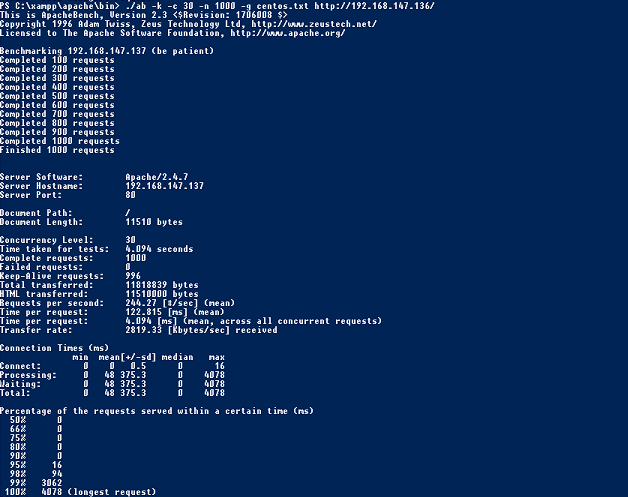
\includegraphics[width=1\linewidth]{ab1.png} 
\caption{Resultados del Benchmark de Apache en CentOS.} 
\label{contexto:figura} 
\end{figure}

\pagebreak

\item Benchmark del Apache en Ubuntu Server.

\begin{figure}[H]
\centering 
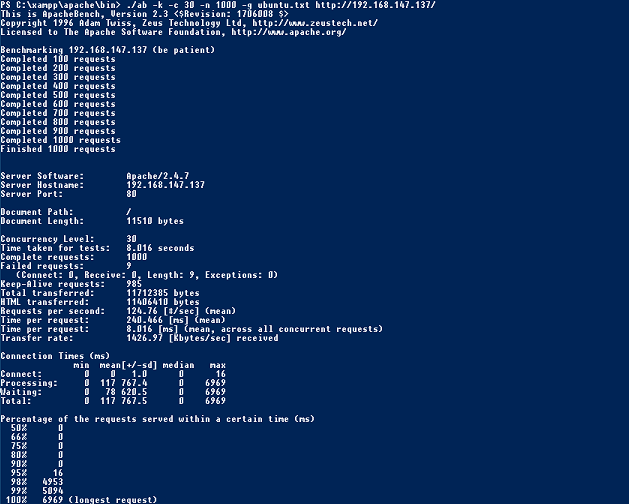
\includegraphics[width=1\linewidth]{ab2.png} 
\caption{Resultados del Benchmark de Apache en Ubuntu Server.} 
\label{contexto:figura} 
\end{figure}

\pagebreak

\item Benchmark del IIS en Windows Server.

\begin{figure}[H]
\centering 
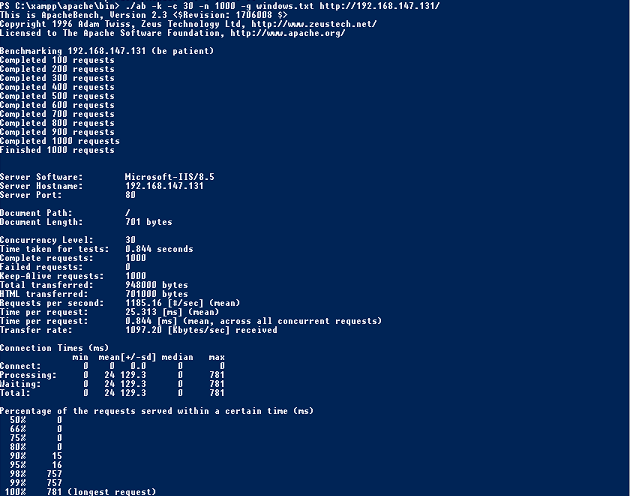
\includegraphics[width=1\linewidth]{ab3.png} 
\caption{Resultados del Benchmark de IIS en Windows Server.} 
\label{contexto:figura} 
\end{figure}

Para facilitar el saber que servidor tiene mejor rendimiento vamos a extraer los datos más significativos en una tabla:

\begin{figure}[H]
\centering 
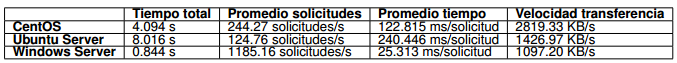
\includegraphics[width=1.1\linewidth]{ab4.png} 
\caption{Tabla comparativa de resultados del Benchmark Apache.} 
\label{contexto:figura} 
\end{figure}

Como podemos ver las diferencias entre los 3 son grandes, tardando CentOs la mitad que Ubuntu Server, pero ambos tardando varios segundos en realizar las 1000 peticiones, mientras Windows Server tardó menos de un segundo en realizar todas las peticiones, siendo el más rápido de todos con diferencia.


\end{itemize}

\pagebreak

\section{Cuestión 4.}
\textbf{Instale y siga el tutorial en \url{http://jmeter.apache.org/usermanual/build-web-test-plan.html} realizando capturas de pantalla y comentándolas. En vez de usar la web de jmeter, haga el experimento usando alguna de sus máquinas virtuales (Puede hacer una página sencilla, usar las páginas de phpmyadmin, instalar un CMS, etc.).}\\

Primero creamos el grupo de hilos:
\begin{figure}[H]
\centering 
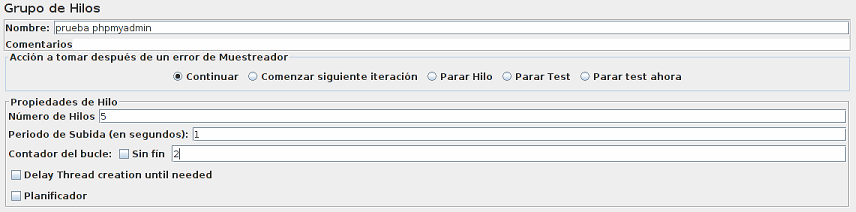
\includegraphics[width=1\linewidth]{jmeter1.png} 
\caption{Creando un grupo de hilos.} 
\label{contexto:figura} 
\end{figure}

Tras esto configuramos la configuración por defecto de cada petición HTTP:
\begin{figure}[H]
\centering 
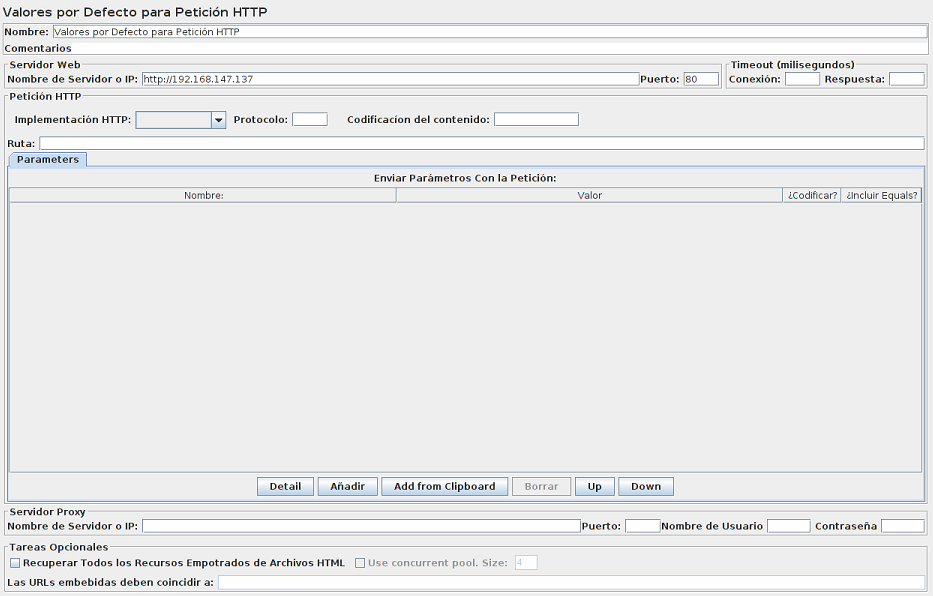
\includegraphics[width=1\linewidth]{jmeter2.png} 
\caption{Cambiando configuración por defecto de petición.} 
\label{contexto:figura} 
\end{figure}

Añadimos soporte de Cookies con:
\begin{verbatim}
Añadir --> Elemento de Configuración --> Gestor de Cookies HTTP
\end{verbatim}

Añadimos la petición HTTP: 
\begin{figure}[H]
\centering 
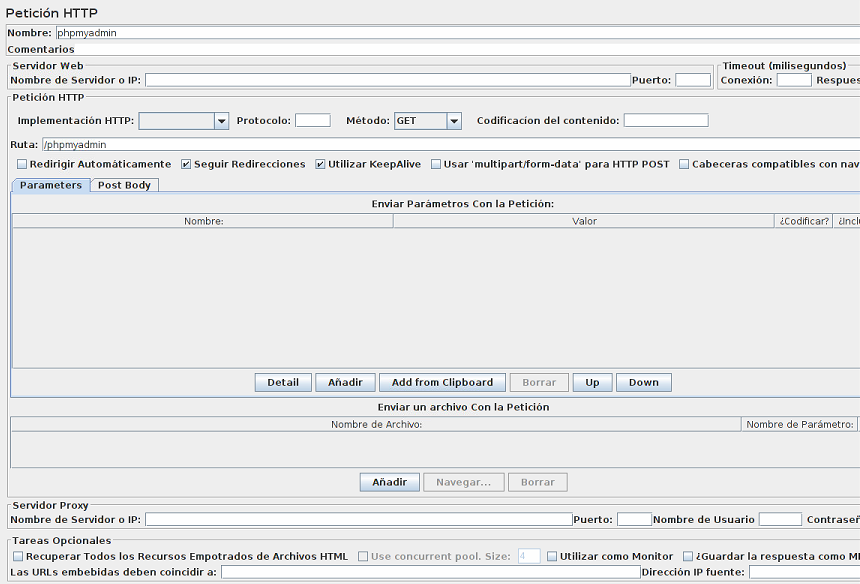
\includegraphics[width=1\linewidth]{jmeter3.png} 
\caption{Añadimos la petición HTTP.} 
\label{contexto:figura} 
\end{figure}

Añadimos una gráfica de escucha con:
\begin{verbatim}
Añadir --> Receptor --> Gráfico de Resultados
\end{verbatim}

Así queda el resultado final:
\begin{figure}[H]
\centering 
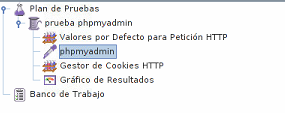
\includegraphics[width=0.8\linewidth]{jmeter4.png} 
\caption{Resultado de la configuración realizada.} 
\label{contexto:figura} 
\end{figure}

\begin{figure}[H]
\centering 
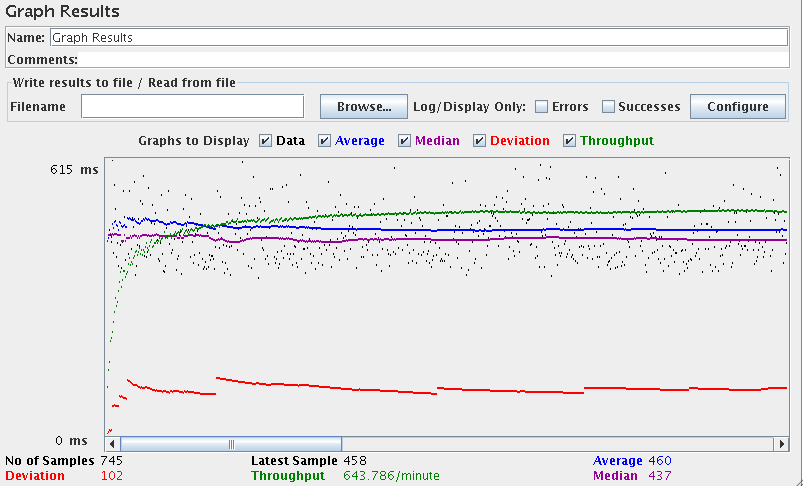
\includegraphics[width=1\linewidth]{jmeter5.png} 
\caption{Gráfica de resultados de la petición.} 
\label{contexto:figura} 
\end{figure}

\pagebreak

\section{Cuestión opcional 4.}
\textbf{Seleccione un benchmark entre SisoftSandra y Aida. Ejecútelo y muestre capturas de pantalla comentando los resultados.}\\

En el caso de benchmark para windows vamos a instalar AIDA64 que se puede descargar de \cite{6}, su instalación es muy sencilla, tan solo ejecutar el archivo \textit{'.exe'} que se ha descargado y se iniciara la instalación. Una vez instalado obtenemos la vista que podemos apreciar en la figura.

\begin{figure}[H]
\centering 
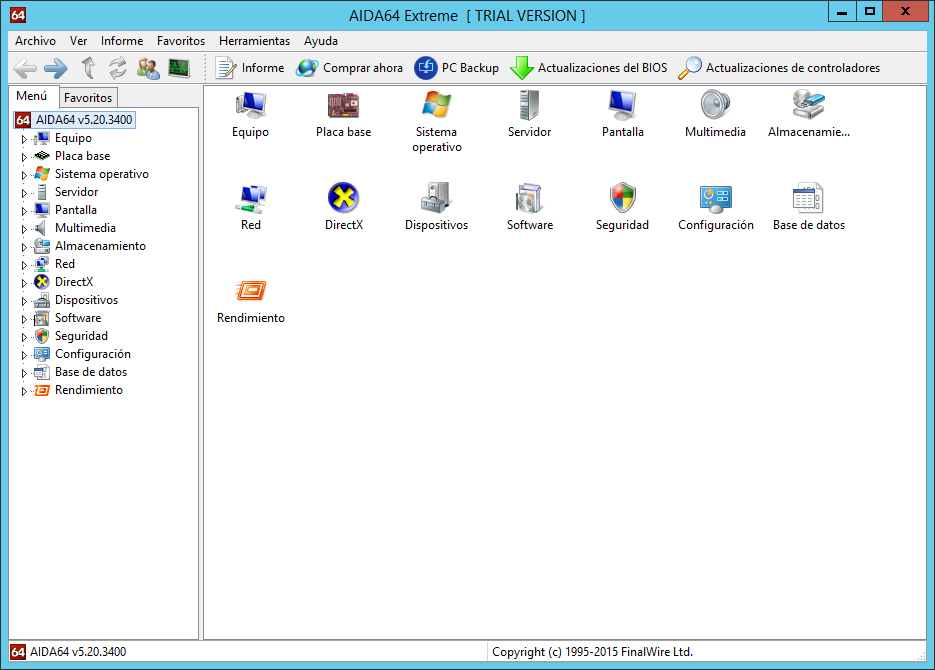
\includegraphics[width=1\linewidth]{aida1.png} 
\caption{Estado final de los discos de sistema.} 
\label{contexto:figura} 
\end{figure}

AIDA64 proporciona varios benchmark de lectura, escritura de memoria y benchmark de CPU, además tiene opciones para crear informes completos con todos estos benchmark realizados por lo que podemos pulsar en la estaña de rendimiento con click derecho presionar en informe rápido y elegir un tipo de salida de forma que se realizarán todos los benchmark, estos benchmark nos permiten comparar el rendimiento de nuestros componentes con otros componentes del mercado y hacernos una idea de lo que tenemos en nuestra máquina por ejemplo en el benchmark de velocidad de lectura se miden las velocidades de escritura en memoria de nuestra máquina para poder compararla con el resto de componentes (figura x).
Además AIDA64 también nos proporciona herramientas como pruebas de rendimiento para cache y memoria (figura x+1) que calcula las velocidades de escritura, lectura de nuestra memoria y caches. (Como es una versión Trial hay datos que no se muestran).

\begin{figure}[H]
\centering 
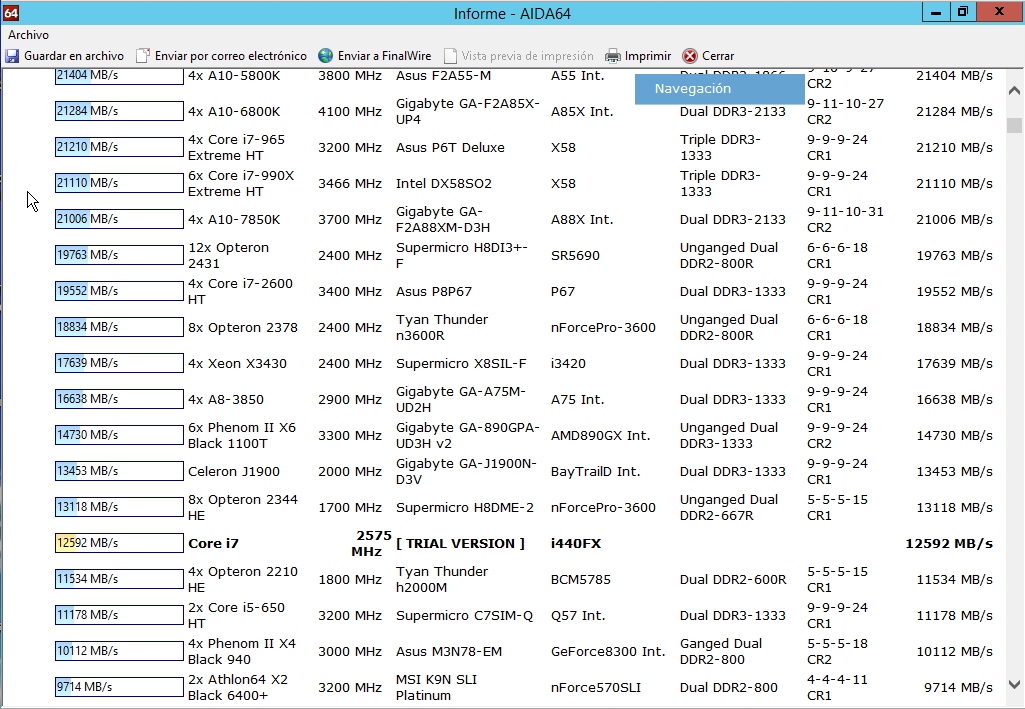
\includegraphics[width=1\linewidth]{aida2.png} 
\caption{Benchmark de Escritura de memoria.} 
\label{contexto:figura} 
\end{figure}    

\begin{figure}[H]
\centering 
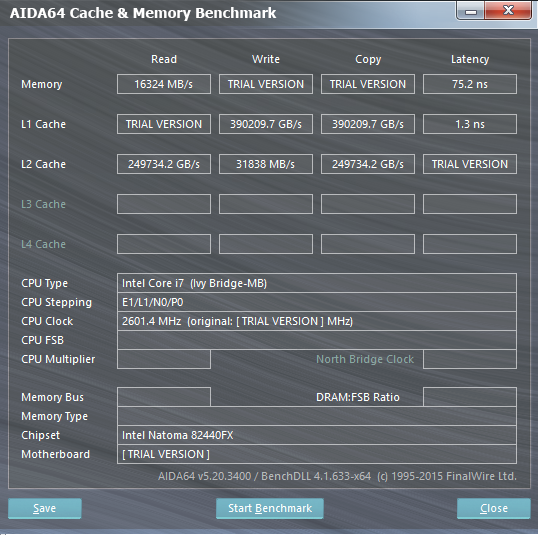
\includegraphics[width=0.5\linewidth]{aida3.png} 
\caption{Benchmark de lectura, escritura de la memoria y caches.} 
\label{contexto:figura} 
\end{figure}

\pagebreak

\section{Cuestión 5.}
\textbf{Programe un benchmark usando el lenguaje que desee. El benchmark debe incluir:
\begin{enumerate}
\item Objetivo del benchmark.
\item Métricas (unidades, variables, puntuaciones, etc.).
\item Instrucciones para su uso.
\item Ejemplo de uso analizando los resultados.
\end{enumerate}
Tenga en cuenta que puede comparar varios gestores de BD, lenguajes de programación web (tiempos de ejecución, gestión de memoria, ...), duración de la batería, servidor DNS, etc., Alternativamente, puede descargar alguno de algún repositorio en github y modificarlo según sus necesidades.}

El recurso sobre el que se va a plantear la hipótesis después de pensarlo, se hará usando memorias extraibles USB por motivos más que obvios como pueden ser la falta de tiempo, y la facilidad de implementación y trabajo físico con el ordenador ya que al no disponer de HDD sata u otros no puedo realizar otro tipo de analisis, aunque el analisis implementado sirve también para HDD sata u extraibles. La idea es hacer una comparativa entre tres elementos, un disco duro extraible que usa puerto USB TrekStor, una memoria USB Alcor 2.0 y una memoria USB Kingston 3.0, para estudiarlos nos interesa obtener datos acerca de la escritura y la lectura de archivos sean grandes o pequeños por eso se han planteado dos experimentos acordes a esta idea:
\begin{itemize}
\item El primer experimento consistirá en medir el tiempo y la velocidad de operaciones de escritura, lectura y una mezcla de dichas operaciones de un archivo con un volumen de 2.0GB.
\item El segundo experimento consistirá en medir el tiempo y la velocidad de operaciones de escritura, lectura y una mezcla de dichas operaciones de muchos archivos (en mi caso 100) cada uno con un volumen de 50 MB lo que viene a corresponder a 5.00 GB aproximadamente.
\end{itemize}

Con respecto a la carga de trabajo, se han elegido estos tamaños puesto que con lo que vamos a trabajar tiene un espacio limitado, y los dispositivos que usan USB 2.0 no son tan rápidos a la hora es escribir archivos grandes por lo que con esos tamaños será más que suficiente para analizar las memorias, para crear dichos archivos hacemos uso de instrucciones de c++ para escribir archivos binarios con el tamaño que se desee. 
Con respecto a las medidas tomadas, se analizará tanto el tiempo de escritura total de los archivos como la velocidad en MB/s. La toma de medidas implementada puede ser un poco molesta por el tiempo que se demora ya que son necesarias una cantidad de datos para realizar las medias y por tanto para la realización de ambos experimentos puede demorarse alrededor de 90 mínutos para que los datos obtenidos sean más fiables.
La hipótesis a la que se quiere llegar realizando estas pruebas es: Los discos duros extraibles tienen mayor velocidad de escritura y lectura que otros dispositivos USB sean 2.0 o 3.0. Para realizar las pruebas se ha realizado el benchmark que se pide implementar, y posteriormente se ha realizado un análisis teórico que se encuentra en la carpeta ''Análisis'' del benchmark. Vamos a comentar los resultados que me parecen más relevantes:\\

\pagebreak

Vamos a comenzar con el experimento 1:
\begin{itemize}
\item \textbf{Escritura en dispositivo:}
Como podemos observar en la figura 17 y por los datos aportados por el benchmark, el tiempo de Escritura en las memoria USB, sea 2.0 o 3.0, es mucho más grande que en el disco Extraible, esto puede ser devido a la estructura hardware de cada elemento, ya que las memorias USB son memorias flash y el disco duro usa platos, por lo que escribir en un plato en una determinada sección es posiblemente más rapido que hacerlo en un dispositivo flash.\\
Tiempos:
\begin{verbatim}
USB3.0	DISCOEXTRAIBLE	USB2.0
	
224,827	73,0471	253,679
238,093	63,5761	270,637
240,019	63,2625	299,595
242,304	61,6963	293,076
242,38	67,9739	314,684

\end{verbatim}
Intervalos de confianza(respectivamente): 
\begin{verbatim}
[228,4385433164, 246,6106566836]
[60,1736212308, 71,6487387692]
[256,3166292447, 316,3517707553]
\end{verbatim}
Velocidades:
\begin{verbatim}
USB3.0	DISCOEXTRAIBLE	USB2.0
	
9,10922	28,0367	8,07319
8,6017	32,2133	7,56734
8,53266	32,373	6,83589
8,45218	33,1949	6,98795
8,44954	30,1292	6,50812

\end{verbatim}
Intervalos de confianza(respectivamente): 
\begin{verbatim}
[8,2866954294, 8,9714245706]
[28,5897085763, 33,7891314237]
[6,4206993818, 7,9682966182]
\end{verbatim}
\begin{figure}[H]
\centering 
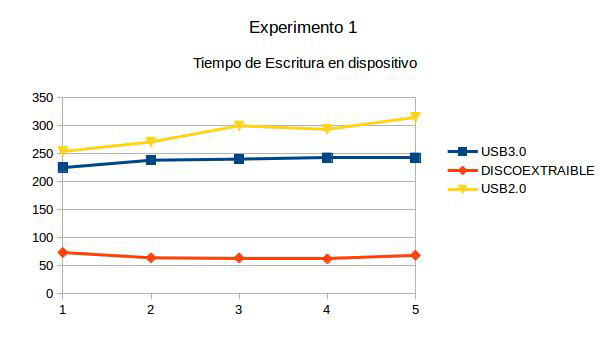
\includegraphics[width=.8\linewidth]{bm1.png} 
\caption{Gráfica de Tiempo de escritura.} 
\label{contexto:figura} 
\end{figure}
\begin{figure}[H]
\centering 
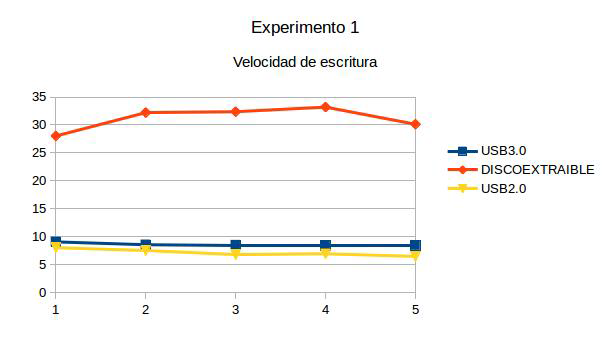
\includegraphics[width=.8\linewidth]{bm2.png} 
\caption{Gráfica de Velocidad de escritura.} 
\label{contexto:figura} 
\end{figure}
\item \textbf{Lectura en dispositivo:} Sin embargo los datos obtenidos nos dicen que las memorias flash 3.0 son más rápidas a la hora de leer un fichero contenido en la misma, esto puede ser por la velocidad de transferencia de los puertos que están preparados para estas unidades 3.0, y por la tardanza del disco en buscar las secciones. (figura 18)\\
Tiempos:
\begin{verbatim}
USB3.0	DISCOEXTRAIBLE	USB2.0

39,2158	85,5879	134,683
37,97	94,0525	134,744
41,489	96,4047	141,512
40,0996	90,4485	140,747
38,7784	93,6922	142,632


\end{verbatim}
Intervalos de confianza(respectivamente): 
\begin{verbatim}
[37,8380588981, 41,1830611019]
[86,8431682756, 97,2311517244]
[134,0863965121, 143,6408034879]

\end{verbatim}
Velocidades:
\begin{verbatim}
USB3.0	DISCOEXTRAIBLE	USB2.0
	
52,2238	23,9286	15,206
53,9373	21,7751	15,1991
49,3625	21,2438	14,4723
51,0728	22,6427	14,551
52,8129	21,8588	14,3586


\end{verbatim}
Intervalos de confianza(respectivamente): 
\begin{verbatim}
[49,7124678733, 54,0512521267]
[20,9942087077, 23,5853912923]
[14,2457254748, 15,2690745252]
\end{verbatim}
\begin{figure}[H]
\centering 
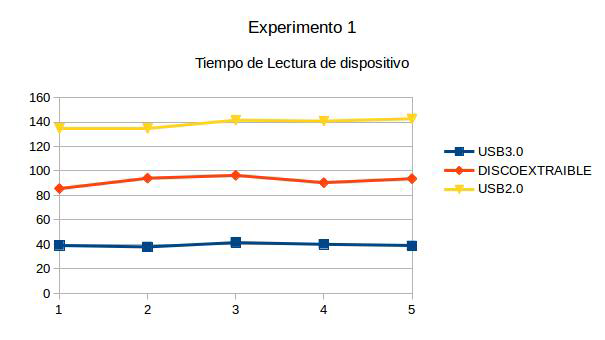
\includegraphics[width=.8\linewidth]{bm3.png} 
\caption{Gráfica de Tiempo de lectura.} 
\label{contexto:figura} 
\end{figure}
\begin{figure}[H]
\centering 
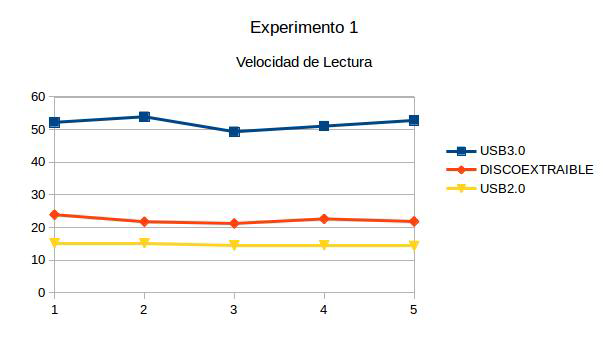
\includegraphics[width=.8\linewidth]{bm4.png} 
\caption{Gráfica de Velocidad de lectura.} 
\label{contexto:figura} 
\end{figure}
\item \textbf{Escritura/Lectura en dispositivo:} La escritura y lectura es una operación alternada entre las dos anteriores sin embargo, es muy similar a la salida que se produce cuando directamente escribimos, parece que el coste en tiempo de lectura de trozos más pequeños mientras se esta escribiendo no tiene un impacto muy grande en tiempo por tanto el disco es el más rápido. 
\end{itemize}

\pagebreak

Vamos a comenzar con el experimento 2:
\begin{itemize}
\item \textbf{Escritura en dispositivo:}
Para la escritura de muchos archivos de tamaño reducido se produce lo mismo que en el experimento 1, el disco duro tiene una estructura que permite una velocidad mayor de escritura pese a que la salida sea 2.0.\\
Tiempos:
\begin{verbatim}
USB3.0	DISCOEXTRAIBLE	USB2.0
	
586,369	157,098	741,888
613,674	164,436	790,578
613,188	160,346	750,954
597,932	154,524	723,0955082
612,581	170,969	765,9485
\end{verbatim}
Intervalos de confianza(respectivamente): 
\begin{verbatim}
[589,585895606, 619,911704394]
[153,4360187715, 169,5131812285]
[722,8939242407, 786,0916790393]

\end{verbatim}
Velocidades:
\begin{verbatim}
USB3.0	DISCOEXTRAIBLE	USB2.0
	
8,52705	31,8273	6,73956
8,14765	30,407	6,32449
8,1541	31,1826	6,65819
8,36215	32,3575	5,23515
8,16219	29,2451	5,27145
\end{verbatim}
Intervalos de confianza(respectivamente): 
\begin{verbatim}
[8,0604695533, 8,4807864467]
[29,4842152052, 32,5235847948]
[5,1268603187, 6,9646756813]

\end{verbatim}
\begin{figure}[H]
\centering 
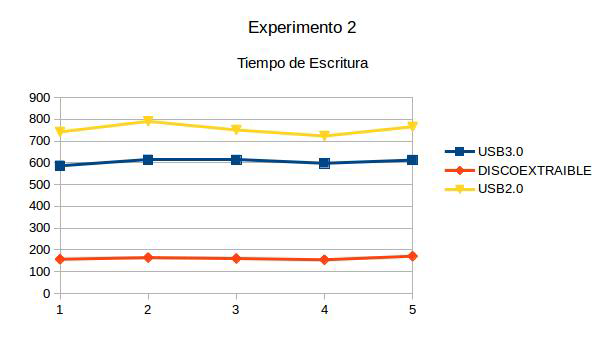
\includegraphics[width=.8\linewidth]{bm5.png} 
\caption{Gráfica de Tiempo de escritura.} 
\label{contexto:figura} 
\end{figure}
\begin{figure}[H]
\centering 
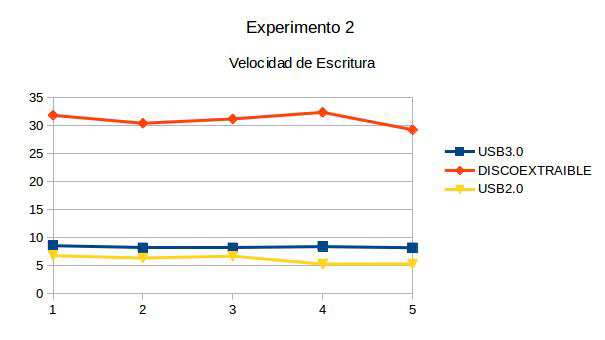
\includegraphics[width=.8\linewidth]{bm6.png} 
\caption{Gráfica de Velocidad de escritura.} 
\label{contexto:figura} 
\end{figure}
\item \textbf{Lectura en dispositivo:} Ocurre exactamente lo mismo que el experimento 1 el USB 3.0 tiene la mejor velocidad y tiempo de lectura. (figura 23)\\
Tiempos:
\begin{verbatim}
USB3.0	DISCOEXTRAIBLE	USB2.0
	
88,3328	215,326	355,336
91,1757	216,5	358,154
88,687	205,875	275,722
88,0768	215,787	295,82826
87,8435	205,924	314,9563



\end{verbatim}
Intervalos de confianza(respectivamente): 
\begin{verbatim}
[87,1445900944, 90,5017299056]
[205,0810190598, 218,6837809402]
[274,9104340972, 365,0881899028]


\end{verbatim}
Velocidades:
\begin{verbatim}
USB3.0	DISCOEXTRAIBLE	USB2.0
	
56,6041	23,2206	14,0712
54,8392	23,0947	13,9605
56,378	24,2866	18,1342
56,7686	23,171	16,03675
56,9194	24,2808	17,2674
\end{verbatim}
Intervalos de confianza(respectivamente): 
\begin{verbatim}
[55,2564035274, 57,3473164726]
[22,8459201016, 24,3755598984]
[13,5722208951, 18,2157991049]
\end{verbatim}
\begin{figure}[H]
\centering 
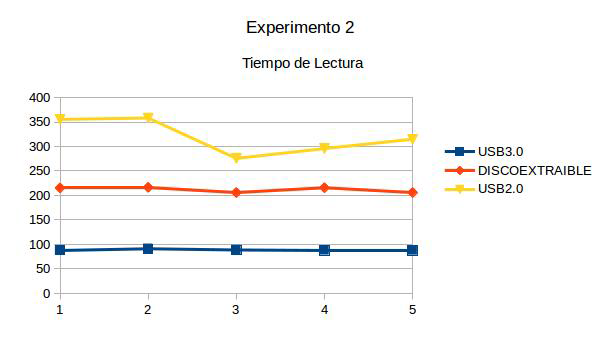
\includegraphics[width=.8\linewidth]{bm7.png} 
\caption{Gráfica de Tiempo de lectura.} 
\label{contexto:figura} 
\end{figure}
\begin{figure}[H]
\centering 
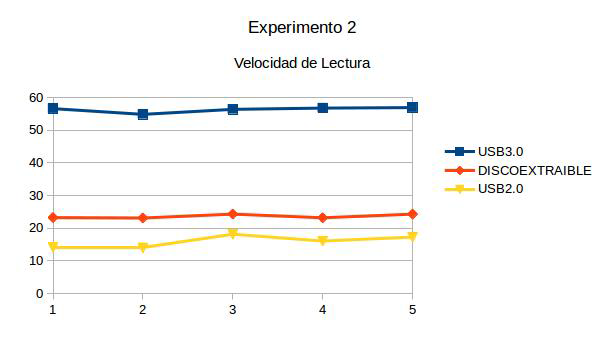
\includegraphics[width=.8\linewidth]{bm8.png} 
\caption{Gráfica de Velocidad de lectura.} 
\label{contexto:figura} 
\end{figure}
\item \textbf{Escritura/Lectura en dispositivo:} Ocurre exactamente lo mismo que en la escritura debido a que se reduce el tiempo de lectura demasiado por lo que no se produce un impacto muy fuerte en el tiempo total de escritura y lectura. 
\end{itemize}
\textbf{Conclusión:} En mi opinion hemos probado la hipótesis en parte, ya que es cierto que para estos tres dispositivos el disco duro tiene una mayor velocidad de escritura (menor tiempo) que el resto de dispositivos, sin embargo el usb 3.0 lo supera en la velocidad de lectura. Aunque finalmente cuando vamos a usar un disco duro extraible nos interesa normalmente que se produzcan operaciones de lectura y escritura entremezcladas por lo que un disco duro extraible es mejor opción que un usb3.0 por esa misma razón, ya que como se ha indicado antes el impacto de tiempo de la lectura sobre las operaciones de escritura es muy pequeño normalmente y permite mejores tiempo al disco duro extraible.

\pagebreak

La programación del Benchmark se ha llevado a cabo haciendo uso del lenguaje c++, implementando una clase que se dedica ha hacer el análisis de unidades de almacenamiento. El análisis de los resultados se lleva a cabo de manera manual por motivos de tiempo, por defecto el programa implementado aporta una versión de los datos en formato cvs, para que pueda ser modificado con un editor estadístico sin embargo es muy probable que tengan que cambiarse las preferencias de lenguaje. El funcinamiento del benchmark es como se describe en la figura 25, en primer lugar se iniciará una instancia de la clase benchmark que será la que ejecute los tests, introducimos el número del experimento que queremos realizar en el caso de introducir uno que no exista se volverá a preguntar, es importante mencionar que este diagrama se producirá tantas veces como niveles se quieran hacer, en nuestro caso 3, despues de haber seleccionado el experimento se preguntará cual es el nombre del dispositivo conectado al usb y posteriormente se realizarán los tres tests de escritura, lectura y una alternada de ambas operaciones. Estos tests se realizarán 5 veces y por último se calculará la velocidad a partir del tiempo y se copiarán los datos a un archivo cvs.\\
El benchmark implementado actua de forma independiente, tan solo se pide al usuario introducir el nombre del dispositivo a analizar cada cierto tiempo.
\begin{figure}[H]
\centering 
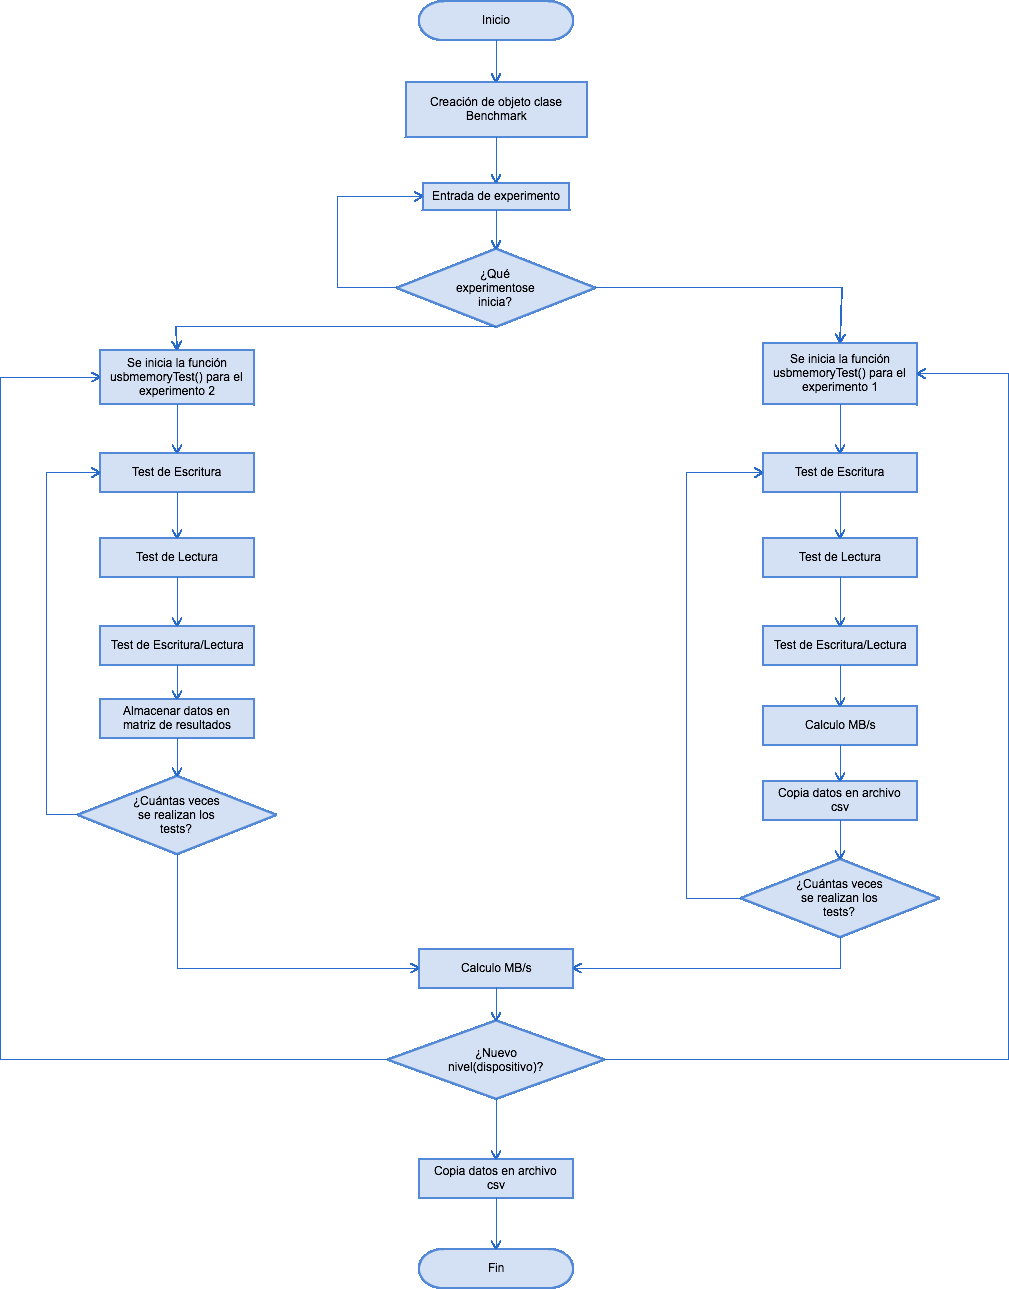
\includegraphics[width=.72\linewidth]{fchart.png} 
\caption{Diagrama de Flujo del programa que ejecutará la prueba de rendimiento.} 
\label{contexto:figura} 
\end{figure}

\textbf{Esquema de subdirectorios del archivo comprimido:}
\begin{itemize}
\item benchmark
\begin{itemize}
\item Análisis
\begin{description}
    \item Exp1.ods
	\item Exp2.ods
	\item Exp1.csv
	\item Exp2.csv
\end{description}
\item bin
\begin{description}
	\item Bench
\end{description}
\item include
\begin{description}
	\item benchmark.h
\end{description}
\item object
\item src
\begin{description}
	\item benchmark.cpp
	\item main.cpp
\end{description}
\item data.csv
\item infousb
\end{itemize}
La salida del programa se realiza en data.csv, los archivos de la carpeta Análisis contienen el análisis teórico de los datos resultantes del benchmark en los archivos Exp1.ods y Exp2.ods, la carpeta bin contiene el archivo binario tal y como se espera, include las cabeceras y src el código del programa.
\end{itemize} 

\pagebreak

\begin{thebibliography}{99}
\bibitem{1} \url{http://www.phoronix-test-suite.com/documentation/phoronix-test-suite.pdf}
\bibitem{2} \url{http://fedoraproject.org/wiki/EPEL/es}
\bibitem{3} \url{http://www.phoronix.com/scan.php?page=news_item&px=NzA3Mg}
\bibitem{4} \url{http://www.phoronix-test-suite.com/?k=documentation}
\bibitem{5} \url{https://httpd.apache.org/docs/2.2/programs/ab.html}
\bibitem{6} \url{www.aida64.com/downloads}
\end{thebibliography}
\end{document}
